\section{Implicit General Rules of Counterpoint}

\paragraph{}In this section, all the following rules are implicit, sometimes taken from Fux's examples, and sometimes from music theory in general.

\subsection{Formalization in English} \label{sec:generalenglish}
\begin{enumerate}[wide, label=\bfseries G\arabic*]
    \item \textit{Harmonic intervals are always calculated from the lower note.} \label{rule:hfromlower}

    Indeed, any harmonic interval is a calculation of the absolute difference between two notes. This implies that they adapt to where the counterpoint is in relation to the \cfdot.

    \item \textit{The number of measures of the counterpoint must be the same as the number of measures of the \cfdot} \label{rule:sameNbMeasures}

    The goal is to compose complete counterpoints which last the same time as the \cfdot

    \item \textit{The counterpoint must have the same time signature and the same tempo as the \cfdot} \label{rule:sameTimeSignature}

    The notes must be played in sync.

    \item \textit{The counterpoint must be in the same key as the \cfdot}\label{rule:samekey}

    This is a fundamental rule of music in general. Since the music of the Baroque period does not follow the same standards as today's music, this rule is a bit more complicated than it seems. Indeed, it often happens that Fux gives examples with accidentals, i.e. notes that do not belong to the diatonic scale. There are therefore notes "borrowed" from other scales which do not appear as a basis for the key signature.
    \begin{figure}[h]
        \centering
        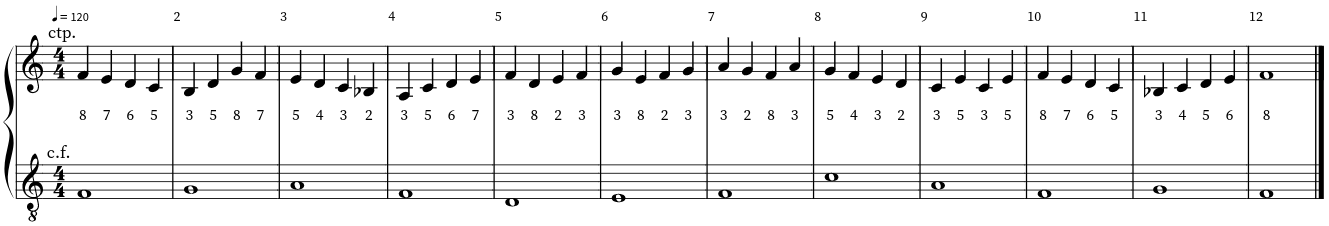
\includegraphics[width=\textwidth]{Images/mode_deter_by_first_note.png}
        \caption{Example of a $C$ major key signature starting on $F$ with $B\flat$'s \parencite[p.54]{GaPEng}.}
        \label{fig:mode_determined}
    \end{figure}

    This makes it somewhat difficult to determine the precise domain of notes available for counterpoint. It is possible to determine the logic behind these borrowed notes. One way of looking at it is as follows: Fux composes with several different modes throughout his work: the $F$ (Lydian) mode, the $D$ (Dorian) mode, and others. In the rules of the first species (see section \ref{subsec:1SPEnglish} at \ref{rule:keytone}), it will be seen that Fux determines the use of a mode according to the first note of the \cf in relation to the key of the musical work. Since the nature of a mode can be either major or minor, some notes can be borrowed from the major or minor diatonic scale of the first note of the \cf respectively.

    In figure \ref{fig:mode_determined}, the key is $C$ major, i.e. [$C, D, E, F, G, A, B$]. These notes can therefore be used in counterpoint, but that is not all. Since the first note is an $F$, this implies that the tonic of this work is $F$, although it uses the major scale of $C$, so it is an example of the use of the $F$ mode, the Lydian mode. The Lydian mode being a major mode, some notes of the diatonic major scale of $F$ can be used sparingly by counterpoint. Looking at several examples given by Fux, the notes borrowed are I ([$F$]\footnote{Notes corresponding to the example are put in square brackets.} necessarily included since it determines the tonic of the work), IV ([$B \flat$] the fourth), VI ([$D$] note of the relative minor) and VII ([$E$] the sensible which is most often used in the penultimate measure). These notes are probably not arbitrary, but for the purposes of this work, it is simply the examples provided by Fux that allow to say that these notes can be used sparingly if necessary.

    If the key notes and the borrowed notes are merged, then the following set of notes is got: [$C, D, E, F, G, A, B \flat, B$]. Since the modes are variations of the diatonic scale, only a few notes are added in the end (one in this case).
    It is more complicated to understand when exactly these borrowed notes are used. Fux explains that these notes can be used to avoid certain intervals at certain times, which otherwise the melody would harshly imply the relationship of \textit{mi} against \textit{fa} \parencite[p.35]{GaPEng}. Again, his approach to music is probably stricter than the current one, especially when his music was intended to be religious songs. That is why this setting is user-definable.

    \item \textit{The range of the counterpoint must be consistent with the instrument used.} \label{rule:instrurange}

    This rule is relatively arbitrary and should be managed by the software user. Fux's treatise is mainly concerned with sung counterpoint, although it is applicable to any instrument. Most of the time, counterpoint is composed either in a higher register or in a lower register and more rarely both simultaneously. For performance reasons, the range in the software is limited to a size of one and a half octaves, i.e. 18 semitones. Which is in itself completely consistent with the style of counterpoint. The user still has the choice of the general pitch of the generated melody.

    \item \textit{Chromatic melodies are forbidden.}\label{rule:chromafb}

    In this work, a melody is considered chromatic when three notes in a row are separated by semitones in the same direction. For example, $C\to C\sharp\to D$ or $C\to B\to B\flat$ are chromatic melodies. As a rule, this should never happen because the diatonic scale does not have those intervals. However, it might be possible to compose chromatic melodies by using borrowed notes in the use of certain modes.
    
    \item \textit{Melodic intervals should be small.}\label{rule:smallmelody}

    The purpose of a melody is to be melodious, but how to define that? This question is several centuries old and still does not have an answer that suits everyone.
    % Some people see melody as a rapid sequence between tension and rest \parencite{Melody}. Others think that the repetition of a motif is essential. Depending on the musical context, it is impossible to define precise rules that work for sure. It is therefore important to see these rules as advices rather than as absolute rules. But how do you represent advice with constraints? One solution is to promote some intervals over others.\\
    In his treatise, Fux argues that one should never neglect the beauty of singing. As a result according to his examples, most melodies consist of stepwise\footnote{Which moves by scale steps (i.e. one tone or one semitone)\parencite{Step}.} motions with occasional leaps. One solution to represent this is to a give higher cost to larger melodic intervals. The appropriate cost function will be discussed in each chapter of species.
    
    % \item \textit{Penultimate notes of the counterpoint tend to rise.} \label{rule:penultrise}

    % While at the end the \cf tends to fall, the counterpoint tends to rise. It makes sense because the last motion must always be contrary (or oblique as will be seen in the next chapter). In Fux's examples, most of them tend to confirm this trend for the last two or even three notes of the counterpoint depending on the species. The examples given in this thesis are therefore strongly influenced by this idea which is omnipresent in the \citetitle{GaPFr}.
\end{enumerate}

\subsection{Formalization into Constraints}

\paragraph{\ref{rule:hfromlower}} \textit{Harmonic intervals are always calculated from the lower note.}

Already handled by making the difference value absolute as seen in section \ref{sec:variables} for the \textbf{H} variable. 

\paragraph{\ref{rule:sameNbMeasures}, \ref{rule:sameTimeSignature}} \textit{Same number of measures and same time signature.}

Only 4/4 time signatures are currently considered. The array $Cp$ is therefore composed of four lists as explained in section \ref{sec:variables} at \textbf{Cp}.

\begin{lstlisting}[caption=Definition of $Cp$ in the first species., label=lst:defcp, basicstyle=\ttfamily\small]
(defvar *cp (list nil nil nil nil))
; ...
;; FIRST SPECIES ;;
; setting the first list of *cp with
;   integer *cf-len as size
;   set *extended-cp-domain as available notes
(setf (first *cp)
    (gil::add-int-var-array-dom *sp* *cf-len *extended-cp-domain))
\end{lstlisting}

\paragraph{\ref{rule:samekey}} \textit{The counterpoint must be in the same key as the \cfdot}

This rule is already handled by the creation of the set $\N$ as shown in section \ref{sec:variables}. The example of the actual rule given above will clarify the explanations. Let $k$ be the value of the key determined by the key signature, i.e. $60$ for $C$; and $t$ the tonic of the piece, i.e. $Cf[0]=65$. Then:

\begin{equation*}
    \begin{gathered}
        \N_{key} = buildScale(k\ mod\ 12, "major") = \{0, 2, 4, 5, 7, 9, 11, 12, \dots, 127\}\\
        \N_{brw} = buildScale(t\ mod\ 12, "borrowed") = \{2, 4, 5, \textbf{10}, 14, \dots, 125\}\\
        \therefore \N_{all}=\{0, 2, 4, 5, 7, 9, \textbf{10}, 11, 12, \dots, 127\}
    \end{gathered}
\end{equation*}

To ensure that borrowed notes are used sparingly, they must be given a cost to use. Let $OffKey$ be the set of notes outside the key and $OffKey_{costs}$ the list of costs associated with each note. The cost for a note will be \textit{<no cost>} or $cost_{OffKey}$ (\dft{high cost}).

\begin{equation}
    \begin{gathered}
        OffKey = [0, 1, 2, \dots, 127] \setminus \N_{key}\\
        % \forall c \in OffKey_{costs}, \forall p \in Cp \\
        % \forall \rho \in \mathcal{P}ositions\\
        \forp\\
        OffKey_{costs}[\rho] = \begin{cases}
            cost_{OffKey} & \text{if } Cp[\rho] \in OffKey \\
            0 & \text{otherwise}
        \end{cases}\\
        \text{moreover } \C = \C \cup \sum _{c \in OffKey_{costs}} c
    \end{gathered}
\end{equation}

This equation is trivial but requires several adjustments in the program. Indeed, there is no boolean constraint in Gecode that assign the value \emph{true} to a variable if an element belongs to a set\footnote{To our knowledge, Gecode provides only a constraint such that an element must be a member of a certain set. Ideally, we would need a reified version of this constraint to allow a boolean associated with the result.}. This can be solved by creating the following constraints (see code sample \ref{lst:is-member-cst}). The idea is to add a 1 each time the candidate element $\equiv$ a member of the set. If the sum of this list $\geq$ 1 then the candidate appears at least once in the set.

\begin{lstlisting}[caption=Function that constrains b-member to be true if candidate is in member-list., label=lst:is-member-cst, basicstyle=\ttfamily\scriptsize]
(defun add-is-member-cst (candidate member-list b-member)
    (let (
        (results (gil::add-int-var-array *sp* (length member-list) 0 1)) ; where candidate == m
        (sum (gil::add-int-var *sp* 0 (length member-list))) ; sum(results)
    )
        (loop for m in member-list for r in results do
            (let (
                (b1 (gil::add-bool-var *sp* 0 1)) ; b1 = (candidate == m)
            )
                (gil::g-rel-reify *sp* candidate gil::IRT_EQ m b1) ; b1 = (candidate == m)
                (gil::g-ite *sp* b1 ONE ZERO r) ; r = (b1 ? 1 : 0)
            )
        )
        (gil::g-sum *sp* sum results) ; sum = sum(results)
        (gil::g-rel-reify *sp* sum gil::IRT_GR 0 b-member) ; b-member = (sum >= 1)
)   )
\end{lstlisting}

\paragraph{\ref{rule:instrurange}} \textit{The range of the counterpoint must be consistent with the instrument used.}

This rule is already handled by the creation of the set $\N^{\R} = \N \cap \R$ as shown in section \ref{sec:variables}. When $Cp$ is created its domain is set to $\N_{all}^{\R}$ as seen in the code sample \ref{lst:defcp}: \texttt{*extended-cp-domain} refers to the set $\N_{all}^{\R}$.

\paragraph{\ref{rule:chromafb}} \textit{Chromatic melodies are forbidden.}

A three-note melody is chromatic if the interval between the first, second and third notes is one semitone in the same direction each time. This can be translated into the two following constraints.

\begin{equation}
    \begin{gathered}
        \forpmm\\
        (M_{brut}[\rho] = 1 \land M_{brut}[\rho+1] = 1) \iff \bot\\
        (M_{brut}[\rho] = -1 \land M_{brut}[\rho+1] = -1) \iff \bot\\
    \end{gathered}
\end{equation}

\begin{lstlisting}[caption=Function that prevents chromatic melodies., label=lst:chromafb-cst]
; add melodic interval constraints such that there is no chromatic interval:
;   - no m1 == 1 and m2 == 1 OR
;   - no m1 == -1 and m2 == -1
; @m-intervals-brut: list of all the melodic intervals
(defun add-no-chromatic-m-cst (m-intervals-brut)
    (loop
        for m1 in m-intervals-brut
        for m2 in (rest m-intervals-brut) do
        (let (
            (b1 (gil::add-bool-var *sp* 0 1)) ; s.f. (m1 == 1)
            (b2 (gil::add-bool-var *sp* 0 1)) ; s.f. (m2 == 1)
            (b3 (gil::add-bool-var *sp* 0 1)) ; s.f. (m1 == -1)
            (b4 (gil::add-bool-var *sp* 0 1)) ; s.f. (m2 == -1)
        )
            (gil::g-rel-reify *sp* m1 gil::IRT_EQ 1 b1) ; b1 = (m1 == 1)
            (gil::g-rel-reify *sp* m2 gil::IRT_EQ 1 b2) ; b2 = (m2 == 1)
            (gil::g-op *sp* b1 gil::BOT_AND b2 0) ; not(b1 and b2)
            (gil::g-rel-reify *sp* m1 gil::IRT_EQ -1 b3) ; b3 = (m1 == -1)
            (gil::g-rel-reify *sp* m2 gil::IRT_EQ -1 b4) ; b4 = (m2 == -1)
            (gil::g-op *sp* b3 gil::BOT_AND b4 0) ; not(b3 and b4)
)   )   )
\end{lstlisting}

The previous function takes care of setting this constraint using GiL. This is a classical example that shows how constraints on all notes of the counterpoint are set when there is no distinction to be made between beats. In this case, \texttt{m-intervals-brut} always represent all the melodic intervals of the counterpoint and not the melodic intervals of a single beat as will often be the case later on. Indeed, one must always adapt to the rule to make it as simple as possible.

The functions often all look the same, a \texttt{let} block declaring the local variables, which are often all the booleans required to determine a situation. Then comes the execution block where the constraints determining the booleans (\texttt{g-rel-reify}) and the restrictive constraints (\texttt{g-op} states that \texttt{b1} and \texttt{b2} must not happen) are set. In the end, putting several constraints one after the other is the same thing as having these same constraints gathered in one separated by $\lor$.

\paragraph{\ref{rule:smallmelody}} \textit{Melodic intervals should be small.}

Just a global minimization of the melodic intervals could be asked to Gecode during the search for solutions but this would not be fully consistent with the stepwise principle. Having a stepwise melody considers that an interval of a semitone is worth the same as having one of a whole tone. It was decided to give the user full control over the costs of the melodic intervals. Indeed, the latter largely determine the melodies produced by the tool. From Fux's examples, the default costs for melodic intervals would be:
\begin{itemize}
    \item the second intervals with no cost;
    \item the third, fourth and octave\footnote{The melodic octave interval is important to be able to quickly return to a comfortable pitch.} intervals with \dft{low cost};
    \item the other intervals with \dft{medium cost}.
\end{itemize}

\begin{equation}\label{eq:mdeg_costs}
    \begin{gathered}
        \forpm\\
        Mdeg_{costs}[\rho] = \begin{cases}
            cost_{secondMdeg} & \text{if } M[\rho] \in \{0, 1, 2\}\\
            cost_{thirdMdeg} & \text{if } M[\rho] \in \{3, 4\}\\
            cost_{fourthMdeg} & \text{if } M[\rho] = 5\\
            cost_{tritoneMdeg} & \text{if } M[\rho] = 6\\
            cost_{fifthMdeg} & \text{if } M[\rho] = 7\\
            cost_{sixthMdeg} & \text{if } M[\rho] \in \{8, 9\}\\
            cost_{seventhMdeg} & \text{if } M[\rho] \in \{10, 11\}\\
            cost_{octaveMdeg} & \text{if } M[\rho] = 12\\
        \end{cases}\\
        \text{moreover } \C = \C \cup \sum _{c \in Mdeg_{costs}} c
    \end{gathered}
\end{equation}

The case of the melodic tritone will be explained later in rule \ref{rule:notritone}.

% \paragraph{\ref{rule:penultrise}} \textit{Penultimate notes of the counterpoint tend to rise.}

% It is mostly a self-created trend due to other constraints. So there is no constraint to put on it because it is only a consequence of the next ones. Nevertheless, it is necessary to have it in mind in order to understand certain subtleties that are coming.